%%%%%%%%%%%%%%%%%%%%%%%%%%%%%%%%%%%%%%%%%
% Journal Article
% LaTeX Template
% Version 1.4 (15/5/16)
%
% This template has been downloaded from:
% http://www.LaTeXTemplates.com
%
% Original author:
% Frits Wenneker (http://www.howtotex.com) with extensive modifications by
% Vel (vel@LaTeXTemplates.com)
%
% License:
% CC BY-NC-SA 3.0 (http://creativecommons.org/licenses/by-nc-sa/3.0/)
%
%%%%%%%%%%%%%%%%%%%%%%%%%%%%%%%%%%%%%%%%%

%----------------------------------------------------------------------------------------
%	PACKAGES AND OTHER DOCUMENT CONFIGURATIONS
%----------------------------------------------------------------------------------------

\documentclass[12pt,twoside,twocolumn]{article}


\usepackage{amsthm}
\usepackage{amsmath}
\usepackage{dsfont}
\usepackage{xcolor}
\usepackage{graphicx}

\usepackage{blindtext} % Package to generate dummy text throughout this template 

\usepackage[sc]{mathpazo} % Use the Palatino font
\usepackage[T1]{fontenc} % Use 8-bit encoding that has 256 glyphs
\linespread{1.08} % Line spacing - Palatino needs more space between lines
\usepackage{microtype} % Slightly tweak font spacing for aesthetics

\usepackage[english]{babel} % Language hyphenation and typographical rules

\usepackage[left=15mm, right=15mm, top=23mm, bottom=24mm, columnsep=9mm]{geometry} % Document margins
\usepackage[hang, small,labelfont=bf,up,textfont=it,up]{caption} % Custom captions under/above floats in tables or figures
\usepackage{booktabs} % Horizontal rules in tables

\usepackage{lettrine} % The lettrine is the first enlarged letter at the beginning of the text

\usepackage{enumitem} % Customized lists
\setlist[itemize]{noitemsep} % Make itemize lists more compact

\usepackage{abstract} % Allows abstract customization
\renewcommand{\abstractnamefont}{\normalfont\bfseries} % Set the "Abstract" text to bold
\renewcommand{\abstracttextfont}{\normalfont\small\itshape} % Set the abstract itself to small italic text

\usepackage{titlesec} % Allows customization of titles
\renewcommand\thesection{\Roman{section}} % Roman numerals for the sections
\renewcommand\thesubsection{\roman{subsection}} % roman numerals for subsections
\titleformat{\section}[block]{\large\scshape\centering}{\thesection.}{1em}{} % Change the look of the section titles
\titleformat{\subsection}[block]{\large}{\thesubsection.}{1em}{} % Change the look of the section titles

\usepackage{fancyhdr} % Headers and footers
\pagestyle{fancy} % All pages have headers and footers
\fancyhead{} % Blank out the default header
\fancyfoot{} % Blank out the default footer
\fancyhead[C]{Preprocessing and Classification of ERD/ERS Signals - Doing by Thinking} % Custom header text
\fancyfoot[RO,LE]{\thepage} % Custom footer text

\usepackage{titling} % Customizing the title section

\usepackage{hyperref} % For hyperlinks in the PDF


%----------------------------------------------------------------------------------------
%	TITLE SECTION
%----------------------------------------------------------------------------------------

\setlength{\droptitle}{-4\baselineskip} % Move the title up

\pretitle{\begin{center}\Huge\bfseries} % Article title formatting
\posttitle{\end{center}} % Article title closing formatting
\title{Preprocessing and Classification of ERD / ERS Signals} % Article title
\author{%
\textsc{Florian Eichin} \\[1ex] % Your name
\normalsize Albert Ludwigs University Freiburg \\ % Your institution
\normalsize \href{mailto:florian.eichin@saturn.uni-freiburg.de}{florian.eichin@saturn.uni-freiburg.de} % Your email address
%\and % Uncomment if 2 authors are required, duplicate these 4 lines if more
%\textsc{Jane Smith}\thanks{Corresponding author} \\[1ex] % Second author's name
%\normalsize University of Utah \\ % Second author's institution
%\normalsize \href{mailto:jane@smith.com}{jane@smith.com} % Second author's email address
}
\date{\today} % Leave empty to omit a date
\renewcommand{\maketitlehookd}{%
\begin{abstract}
\noindent Many modern brain computer interfacing methods rely heavily on the analysis of frequency power of emitted electromagnetic brain signals. Local increase and decrease of power in certain frequency ranges, also referred to as Event Related Synchronization and Desynchronization, has proven to be a feature with very high discriminability for tasks such as classifying imagined left- against right-hand movement with accuracy rates of over 90\%. In practical approaches preprocessing is needed to observe these processes on EEG-signal and reach such high rates. One well known and widely used approach for doing this is an algorithm called Common Spatial Patterns, that determines spatial filters projecting raw EEG-channels into a virtual channel space with optimal contrast in channel power in between two classes for a set of sample epochs.
\end{abstract}
}

%----------------------------------------------------------------------------------------

\begin{document}

% Print the title
\maketitle

%----------------------------------------------------------------------------------------
%	ARTICLE CONTENTS
%----------------------------------------------------------------------------------------
\section{Introduction}

\begin{figure*}
\centering
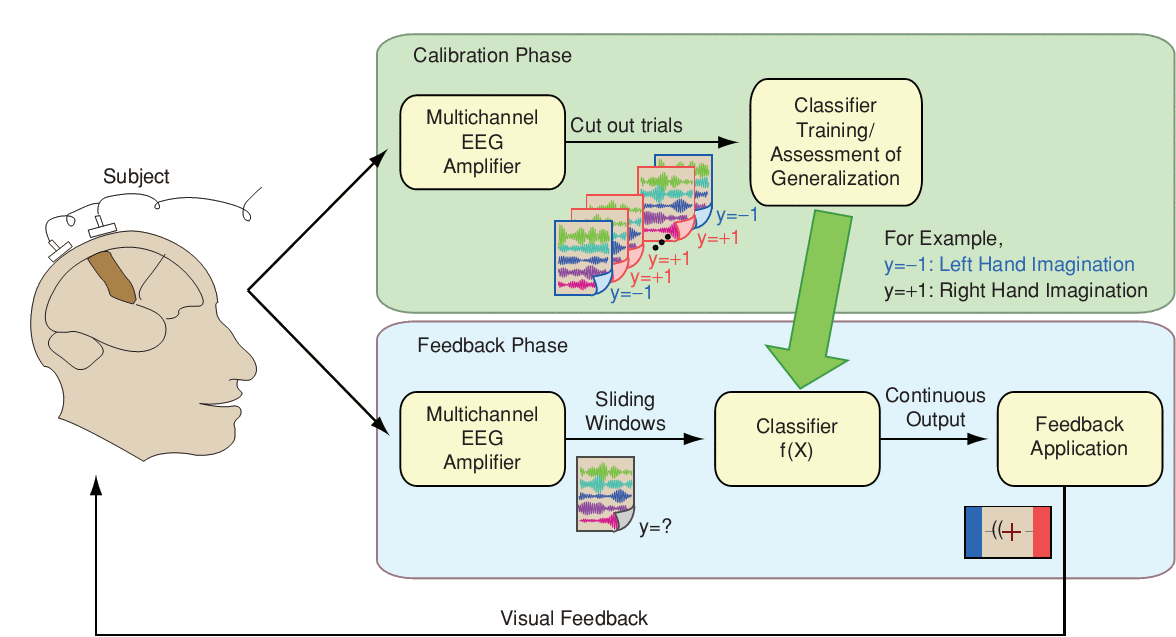
\includegraphics[scale=0.3]{framework.png}
\caption{Overview of the machine-learning-based BCI system. The system runs in two phases. In the calibration phase, we instruct the subjects to perform certain tasks and collect short segments of labeled EEG (trials). We train the classifier based on these examples. In the feedback phase, we take sliding windows from continuous stream of EEG; the classifier outputs a real value that quantifies the likeliness of class membership; we run a feedback application that takes the output of the classifier as an input. Finally the subject receives the feedback on the screen as, e.g., cursor control.}
\end{figure*}

Little is known about the actual processes in the brain, that lead to conscious thinking. However, a basic scheme of which areas of the brain are involved in which tasks is known. There is also a basic understanding, of how "activeness" of parts of the brain can be defined using observations like blood flow, hormone emission and, most prominently, electromagnetic activity of neurons. Several technologies exist to observe these effects of brain activity. They can be used to build brain-computer interfaces, that give information about these phenomena to an application. Usually the process of decoding these phenomena involve several signal processing, digital preprocessing and classification steps. A refresher on all three of these topics can be found in [2]. A basic learning brain computer interface setup can be found in figure 1.

As already noted, the following methods and algorithms can be used to classify between imagined left and right hand movement from brain signals. This task will serve as an example throughout the whole text in order to give intuition and show, what interesting results can be obtained. Of course, the scope of what can be achieved with these methods doesn't end with the comparably basic task of left- against right-hand movement. To get an idea, of what else is possible, a look in [2] will be a good starting point. Also, the reader is expected to have at least a beginner background in machine learning.

This report shall serve as guide through the basic pipeline, that can be used to solve our example task. We will jump into the topic by discussing a basic framework for picking up and working on electromagnetic brain emissions. We will then proceed to discover the underlying brain processes and phenomena, that we want to utilize for solving this classification task and quickly have an overview of the challenges that need to be tackled. In the end we will see two types of spatial filters, called Laplace Filters and Common Spatial Patterns and walk through an approach of putting all the learned concepts together and describe a working classifier for our left/right hand task. 

Please note, that most of the information, that is presented in this report, is based on "Optimizing Spatial Filters for Robust
EEG Single-Trial Analysis" by Benjamin Blankertz (see [1]). Also I want to thank Andreas Meinel, my advisor, for adding a lot to this information and giving me very useful explanations and feedback.

\section{How do we measure brain activity?}
\subsection{Choice of Technology}
A big variety of technologies that measure effects of brain activity are available today. Making a decision for one of these technologies is usually dependent on trade-offs between time and spatial resolution of the retrieved data, as well as costs and mobility of the devices used. In addition to that, we are usually constrained to non-invasive ways of measurement when working with healthy subjects. For a detailed discussion of these technologies, a look into [2] should be again considered.
As already noted, this paper aims at analyzing the power of different frequency bands of electromagnetic brain processes. Thus a method with high time resolution will be needed. The practical benefits of a cheap and mobile solution are also preferable, which is why EEG, out of all the other technologies, will be the method of choice for this talk. Of course most of the concepts presented here can also be applied to other measurement setups, especially spatial filtering is not only useful on EEG-data.

\subsection{Representation of EEG-signals and Channel Names}
For the rest of this talk, we assume that our EEG-signal is sampled in discrete time intervals. With $C \in \mathds{N}$ the number of channels, a sample ${\bf x} \in \mathds{R}^C$ is a vector, where each entry represents the potential of one EEG-channel at a given time point. Subsequent samples ${\bf x}^{(t)}, {\bf x}^{(t+1)}, ..., {\bf x}^{(t+D)} \in \mathds{R}^C$ can be interpreted as epoch-matrix 
\begin{equation}
X = ({\bf x}^{(t)}, {\bf x}^{(t+1)}, ..., {\bf x}^{(t+D)}) \in \mathds{R}^{CxD}
\end{equation}
where $t, D \in \mathds{N}$ are the time point and the duration. 

EEG-electrodes are usually attached on the scalp according to schemes, where each electrode has four neighboring ones. An example of such a scheme can be found in figure 4. Note, that each electrode has a name consisting of one to two letters and a number. The letters usually describe the vertical position (F = "Frontal", C = "Central", P = "Parietal") , the numbers are either zero ("z"), which refers to the middle, even (2, 4, 6) on the right hemisphere and odd (1, 3, 5) on the left.


\section{Oscillatory Analysis}

\begin{figure}
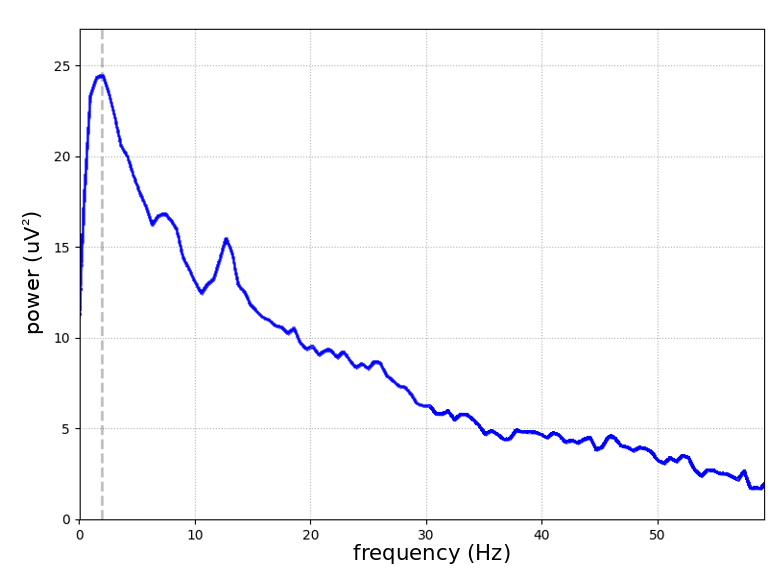
\includegraphics[scale=0.28]{psd.png}
\caption{Mean power spectral density on Pz-channel for resting state EEG-data.}
\end{figure}

\begin{figure*}
  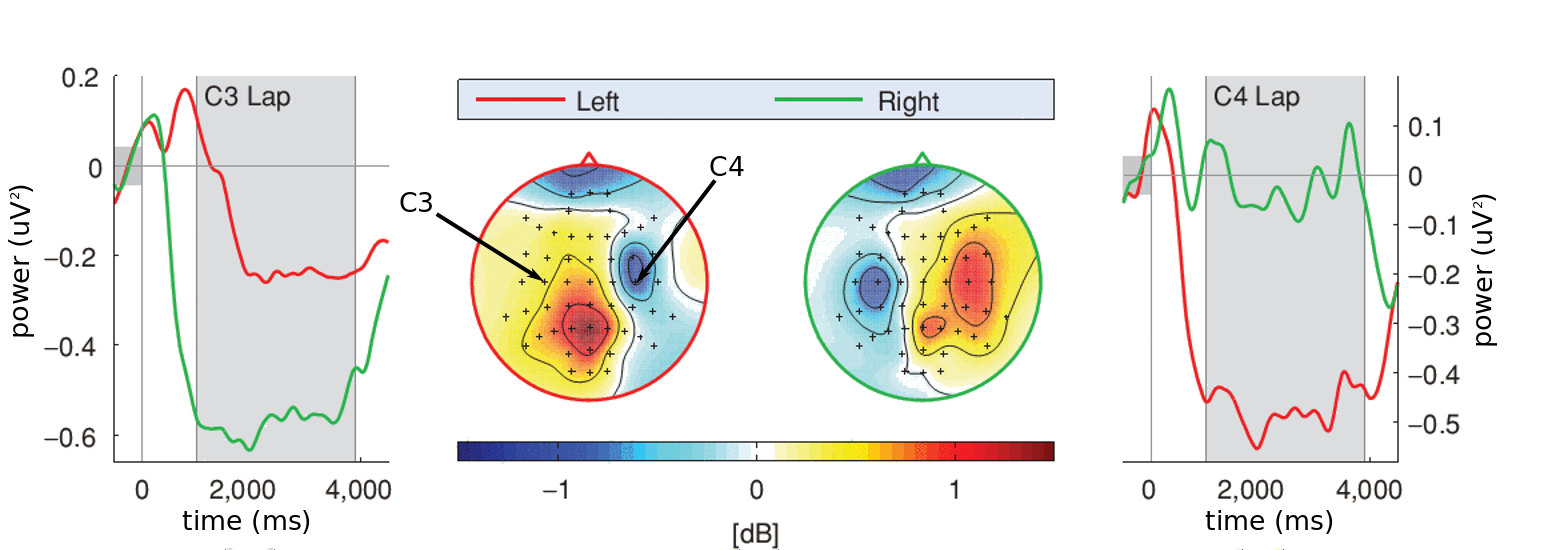
\includegraphics[scale=0.32]{spectralrarr.png}
  \caption{Event-Related Desynchronization (ERD) during motor imagery of the left and the right hand. Raw EEG signals of one subject have been band-pass filtered between 9 and 13 Hz. For the time courses, the envelope of the signals has been calculated by Hilbert transform and averaged over segments of -500 to 4500 ms relative to each cue for left or right hand motor imagery. ERD curves are shown for Laplace filtered channels at C3 and C4, i.e. over left and right primary motor cortex. The topographical maps of ERD were obtained by performing the same procedure for all (non Laplace filtered) channels and averaging across the shaded time interval 1000 to 4000 ms. Source: [1]}
\end{figure*}

Now that the technical framework for this discussion is clarified, we want to shift our attention to the phenomena of brain activity that we will make use of. 
As the header of this section implies, we now want to look at the oscillations of the electromagnetic fields, we can observe on the EEG-signals. 

First we need to clarify, what we can actually pick up with EEG. The largest contributer to electromagnetic brain activity, that we can measure with EEG, are the so called pyramidal nerve cells, that are named after their conic shape. According to [5] these cells contribute to around 80\% of the relevant activity in our EEG-signal. Pyramidal cells are aligned in large groups, orthogonally to the surface of the brain. Whenever we have locally co-activated and co-aligned activity within these populations, their electromagnetic emissions add up. This is when their emissions become strong enough to break through the noise carpet and observable on the EEG. 

There are several known phenomena, that can lead to such a large scale, synchronous activity. One of them is assumed to be connected to local inactivity of the brain. Neurons seem to enter a kind of idle state, whenever they are without task. In these idle states, whole populations of neurons start oscillating in characteristic frequency bands. For example in the sensor- and motor-cortex we can observe the so called $\mu$- and $\beta$-rhythms at 8-15 Hz and 20-35 Hz respectively. Another quiet prominent example is the $\alpha$-rhythm at 8-15 Hz found in the visual cortex. Please have a look at figure 2, that shows an according peak at around 12 Hz in a power spectral density plot, which could be linked to an $\alpha$-rhythm. 

Now, as already indicated, the only thing that can be observed on the EEG, is the increase and decrease of power in certain frequency bands related to certain tasks. In figure 3 we can see such a local increase and decrease of power in the 8-13 Hz range beneath CP3- and CP4-electrodes for left- and right-hand movement. With the assumption, that these observations are connected to idle oscillations, leaving parts of the brain without task, we  call the process of power increasing an Event Related Synchronization (ERS) and a decrease in power an Event Related Desynchronization (ERD).

Keeping in mind, that a lot of motor tasks are linked to certain parts of the brain, we can conclude, that a local ERD/ERS will give us useful information for discriminating between left- and right-hand movement. This is also indicated by figure 3, where we can see a very nice power increase for all electrodes on the right hemisphere for right hand movement. This makes sense, as right hand movement is assumed to be coordinated from the left side of the motor cortex thus leaving the right side in idle state. 

\section{Challenges}
With the results discussed in the previous section, the question of why we actually need to go any further with our investigation arises. The Event Related Synchronizations in figure 3 look already very promising and seem to indicate, that simply the EEG-power of the CP3- and CP4-channels might be enough to discriminate between the two classes of left and right hand movement. However this is not the case as there are  still challenges to tackle in practical approaches. The following section shall give a short introduction to each of them.

EEG data has a rather poor signal-to-noise ratio. This can be traced back to many different noise sources, that can be both external and internal. External noise sources are for example  electrical devices or power lines, as well as the EEG-equipment itself. Internal sources of noise can be muscle artifacts, transpiration and blood flow as well as non task-related brain activity. 

Adding to that, we chose CP3 and CP4 electrodes for detecting local ERD and ERS signals in the last chapter. However these processes have a very high subject-to-subject variation. For the participant these ERD/ERS where detected on, the chosen positions worked very well, but for every new subject we will have to manually search and detect the best positions for observing strong ERD/ERS again. And even this search might not be optimal at all, meaning that just by improving the localization of interesting activity we might improve our results a lot. In addition to that, even with the same subject we will also be confronted with a high session-to-session variation as brain processes are not stationary and slight changes of positions of the electrodes lead to completely different EEG-data.

Finally a common EEG can consist of up to 128 channels of picked up signal. If we want to classify directly on on power features of these channels, we need to train with the same or even higher dimensionality. This usually involves the need for a lot of data, which is usually not available, as we have to rely on short calibration sessions for each new subject and old data is only minor useful for the same reasons that we just discussed for the problem of localization.

\section{Spatial Filtering}
\begin{figure}
\centering
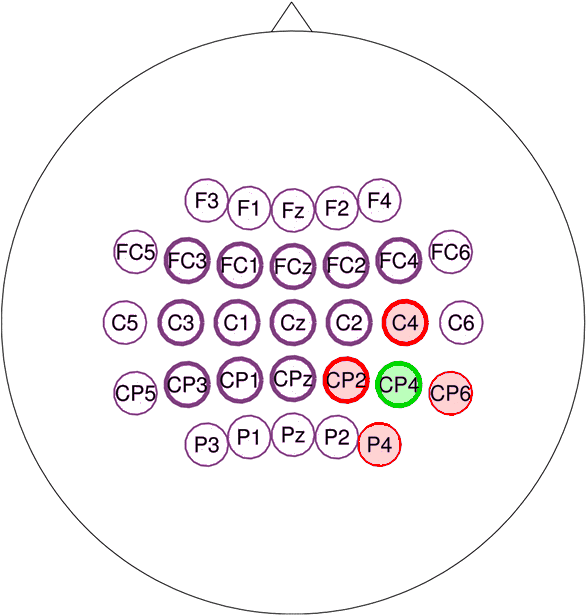
\includegraphics[scale=0.30]{lfilter3.png}
\caption{A basic 31-channel EEG layout. Consider section II.2 for an explanation on the names of the channels. The coloring represents the idea behind a Laplace Filtered CP4-channel, where the mean of the surrounding channels is subtracted from the signal.}
\end{figure}

\begin{figure*}
\centering
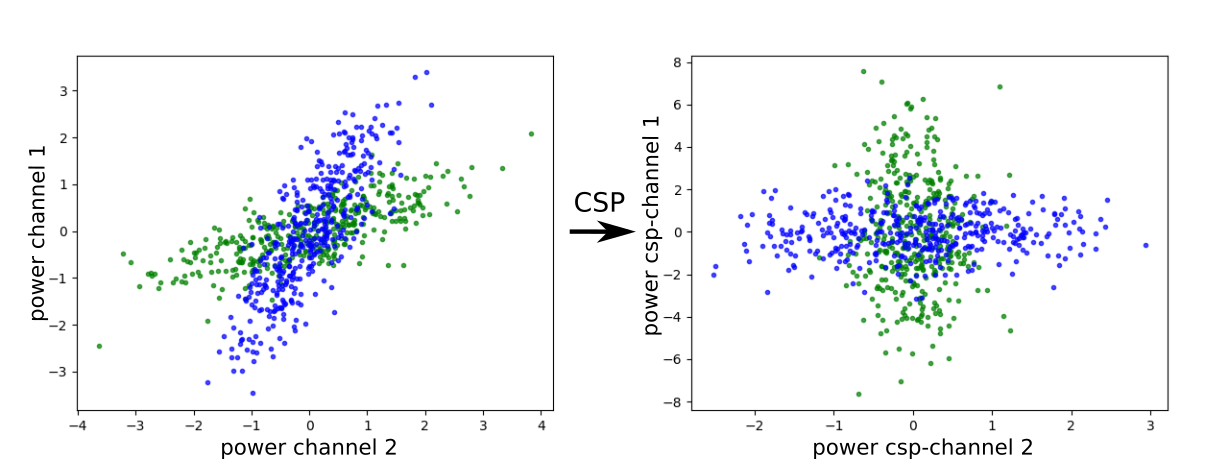
\includegraphics[scale=0.34]{scattered.png}
\caption{On the left: Raw two-channel EEG-samples plotted for two classes L and R. The goal of Common Spatial Patterns is the maximum contrast of variance in the virtual CSP-channels (right side).}
\end{figure*}

In the following we want to explore two different approaches for solving the described problems. Both fall in the class of spatial filters, which can be defined as vectors ${\bf w} \in \mathds{R}^C$, where C is again the number of channels. For a sample ${\bf x} \in \mathds{R}^C$ the filtered sample is defined by 
\begin{equation}
\tilde{x} = {\bf w}^T \cdot {\bf x} \in \mathds{R}
\end{equation}
Note, that for each filter and sample we obtain a one-dimensional new sample creating a new channel of signal. These new channels are often called surrogate or virtual channels, referring to the fact that these new channels don't consist of raw EEG-signal but are rather a weighted sum of many channels.
Let's now look at a simple way of determining filter weights (the filter-entries $w_i$) and see, what we can achieve with this approach.

\subsection{Simple Solution: Laplace Filters}
Laplace Filters mainly aim at canceling out noise by subtracting the spatial average from interesting channels (see figure 4). If we are for example interested in the signal right beyond CP4-electrode, a Laplace Filter would take the CP4-signal and subtract the average of the four surrounding channels, which are in this case C4, CP6, P4 and CP2. So with signal samples
\begin{equation}
{\bf x} = (x_{F3}, ..., x_{C4}, x_{CP2}, x_{CP4}, x_{CP6}, x_{P4})^T
\end{equation}
this filter would be 
\begin{equation}
{\bf w} = (0, ..., 0,\textcolor{red}{-\frac{1}{4}}, \textcolor{red}{-\frac{1}{4}}, \textcolor{green}{1}, \textcolor{red}{-\frac{1}{4}}, \textcolor{red}{-\frac{1}{4}})^T
\end{equation} 
And the filtered signal, that is computed with the dot-product between ${\bf w}$ and ${\bf x}$ is
\begin{equation}
\tilde{x} = {\bf w}^T \cdot {\bf x} =  \textcolor{red}{-\frac{x_{C4} + x_{CP2} + x_{CP6} + x_{P4}}{4}} + \textcolor{green}{x_{CP4}}
\end{equation}

As you can see, this concept is rather simple and straightforward. In addition to that the frequency spectra of the Laplace filtered and raw CP4-channels shown in figure 6 indicate, that the filtered signal adds to discriminability between imagined left and and right hand movement. We thus can conclude, that our signal-to-noise ratio was improved significantly compared to the raw, unfiltered signal. Furthermore, with Laplace Filters the new number of dimensions equals the number of filters we choose. On the other hand, Laplace Filters still don't offer any way of dealing efficiently with the problem of localization, that was introduced in the previous chapter. We still have to pick interesting channels "by hand", which is again time consuming and not optimal. 

\subsection{Data driven approach: Common Spatial Patterns (CSP)}
Common Spatial Patterns is a machine learning approach for determining the weights of spatial filters. The basic idea of Common Spatial Patterns is the contrasting of variance, which can be viewed as an estimator of power, in channels for epochs of two classes for given sample epochs. Keeping our example of classifying left against right hand movement, we will call these classes L and R in the following. In figure 5 you can see an example, of how Common Spatial Patterns works on two channels of EEG. Note, how in both virtual channels the variance is minimal for one class and minimal for the other. With such channels we would be able to discriminate between the two classes by just looking at the CSP-channel power and deciding for the channel with higher power and the according class. 

To formalize this concept, we need a measure of variance and shared variance between the channels, the covariance. Let $X_1, ..., X_k \in \mathds{R}^{CxD}$ be the sample epochs for class h. Then we estimate the {\bf covariance matrix} by
\begin{equation}
	\Sigma_h = \frac{1}{k} \sum_{i=1}^{k}X_i X_i^T
\end{equation}

With $\Sigma_{L}, \Sigma_{R} \in \mathds{R}^{CxC}$ the covariance matrices for classes L and R respectively, we can now formulate the idea of variance contrasting as an optimization problem. We have to subsequently find orthogonal vectors ${\bf w}_i$ for $i \in 1, ..., C $ that satisfy
\begin{equation}
		{\bf w}_i = \underset{{\bf w} \in \mathds{R}^{C}}{argmax}  \  \frac{{\bf w}^T \Sigma_{L} {\bf w}}{{\bf w}^T \Sigma_{R} {\bf w}}
\end{equation}
This formulation is often referred to as Rayleigh Coefficient. Note how the mean variance for class L in the numerator of the coefficient is maximized against the mean variance for class R in the denominator. The first vectors, that we are going find optimizing this, will have a high variance for class L and a low variance for R, because we have to maximize the numerator and minimize the denominator. However, the more we are constrained by searching in the orthogonal space of the vectors that we found before, the lower this coefficient will become. In the last few vectors that we will find, the mean variance for class L will thus be very low and for class R very high. The vectors we find in between will have give us channels with a somewhat equal variance for both classes, that don't add too much to variance contrasting. That's why in practice, these vectors are usually omitted and only an equal number of first and last filters are used as virtual channels for classification.

\begin{figure*}
  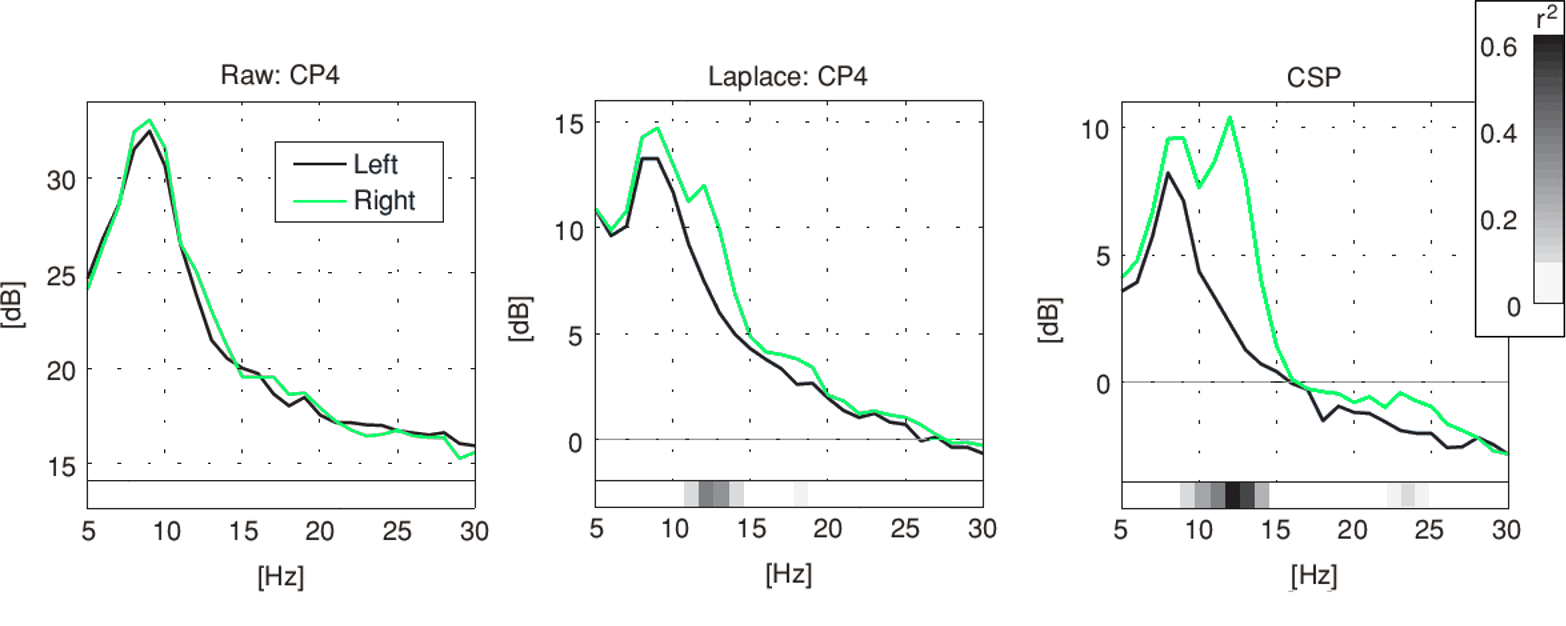
\includegraphics[scale=0.29]{spectracsplp.png}
  \caption{Spectra of left vs. right hand motor imagery. All plots are calculated from the same dataset but using different spatial filters. The discrimination between the two conditions is quantified by the $r^2$-value.}
\end{figure*}

\subsection{Relation of Common Spatial Patterns to Principal Component Analysis}
For those, who already had some experience with machine learning, the above concept might have sounded familiar. That is because the concept of Principal Component Analysis uses a similar concept of variance optimization. Unlike Common Spatial Patterns, Principal Component Analysis does not take the assigned classes for example epochs into account. The optimization problem here for a covariance matrix $\Sigma$ is 
\begin{equation}
		{\bf w}_i = \underset{{\bf w} \in \mathds{R}^{C}}{argmax}  \  \frac{{\bf w}^T \Sigma {\bf w}}{{\bf w}^T{\bf w}}
\end{equation}
Comparing this to the above Rayleigh Coefficient, we can derive, that Common Spatial Patterns is the supervised generalization of Principal Component Analysis. In other words, if class R is uncorrelated, Common Spatial Patterns yields the same filter matrix as Principal Component Analysis for class L. 

This can be easily derived: If class R is uncorrelated, then we have $\Sigma_R = Id$. The Rayleigh Coefficient is then
\begin{equation}
	\underset{w \in \mathds{R}^{N}}{argmax} \frac{w^T \Sigma_{L} w}{w^T \Sigma_{R} w} = \underset{w \in \mathds{R}^{n}}{argmax} \frac{w^T \Sigma_{L} w}{w^T w}
\end{equation}
and we have the optimization criterion for Principal Component Analysis.

\subsection{Analytical Solution for Common Spatial Patterns}
Common Spatial Patterns is, just like Principal Component Analysis, a rare case of a machine learning algorithm with an analytical solution in form of an eigenvalue problem. This makes it even easier to implement the algorithm, as the solving of an eigenvalue problem can be efficiently realized in a few lines of code for many languages. For example in python3's numpy it is one line. Also we will have a much lower runtime compared to doing a gradient search within the optimization problem.

We can reformulate the problem in (7) as
\begin{equation}
{\bf Maximize} \ \textcolor{blue}{{\bf w}^T \Sigma_{L} {\bf w}} \ {\bf w.r.t.} \ \textcolor{purple}{ {\bf w}^T \Sigma_{R} {\bf w} = c}
\end{equation}
where c is a constant. This formulation can be solved using Lagrange Multipliers:
\begin{equation}
	L(\lambda, {\bf w}) =  \textcolor{blue}{{\bf w}^T \Sigma_{L} {\bf w}} - \lambda ( \textcolor{purple}{{\bf w}^T \Sigma_{R} {\bf w} - c})
\end{equation}
To find the critical points, we calculate the first derivative and set it to zero
\begin{equation}
	\frac{\partial}{\partial {\bf w}} L(\lambda, {\bf w}) = 2 \Sigma_{L} {\bf w} - \lambda 2 \Sigma_{R} {\bf w} \overset{!}{=}0
\end{equation}
and if we rearrange this, we get the following
\begin{equation}
	\Sigma_{L} {\bf w} = \lambda \Sigma_{R} {\bf w}
\end{equation}
which is a {\bf generalized eigenvalue problem}. If $\Sigma_R$ is invertible, we can even obtain a normal eigenvalue problem, as it is known it from Linear Algebra I class, by multiplying with $\Sigma_R^{-1}$. 

Now the eigenvectors ${\bf w}_1, ..., {\bf w}_n$ of this problem ordered after their eigenvalues $\lambda_1 > \lambda_2 >...> \lambda_n$ yield the subsequent solutions to our optimization problem and thus the same filters.

If we look at figure 4, we can see, that our new CSP channels give us even better discriminability in terms of $r^2$-score. We can thus derive, that in our virtual channels, we have higher signal-to-noise ratio than with Laplace Filters. Furthermore, the number of filters that we choose is still the number of new channels, meaning, that we can reduce the channel dimensionality as much as we want. Additionally, Common Spatial Patterns is fully automatic and the task of localization is solved without us having to search channels by hand. On the other hand, we're now using a supervised learning algorithm. Before, we had a setup, that worked without the need of labeled training data.  We even have to tune hyperparameters such as the length and time points of the labeled epochs as well as the number of filters we want to us for the classification task. But with the great results in mind and the fact, that we will either way need labeled training data for our classification model, this should not bother us too much.

\subsection{Interpretation of CSP-Filters}
If we take all the vectors ${\bf v}_1, ..., {\bf v}_C \in \mathds{R}^C$ from the eigenvalue spectrum of the Common Spatial Patterns problem, we can put them in a CxC {\bf filter matrix}
\begin{equation}
	W = ({\bf v}_1 ... {\bf v}_C)^T \in \mathds{R}^{CxC}
\end{equation}
which is often referred to as {\bf backward model}, because it maps channels from our raw EEG-signal that was picked up from the scalp back to virtual channels, that are presumed to contain the task related sources of that activity. On the other hand the matrix 
\begin{equation}
	A = W^{-1}
\end{equation}  
is called the forward model, because it maps our virtual channels to the outside, raw signal. The columns of this matrix are also referred to as patterns. If we interpolate the values of the components of filters and patterns to their positions on the scalp, we can obtain informative topographical maps. In figure 7 the filters and patterns with the lowest and highest variance were plotted. As you can see, the filters seem to have a Laplace-like shape, with one extremum on one side of the hemisphere and a a circle shape of weights with inverted sign surrounding it.
The patterns on the other hand have the nice property of having clear, interpretable shapes. They deliver some evidence, of where the channel source can be observed from the outside. Apart from giving us a way of checking the plausibility of our filters, this makes Common Spatial Patterns, apart from being just a preprocessing method, an imaging method with an neurophysiological use.

\begin{figure}
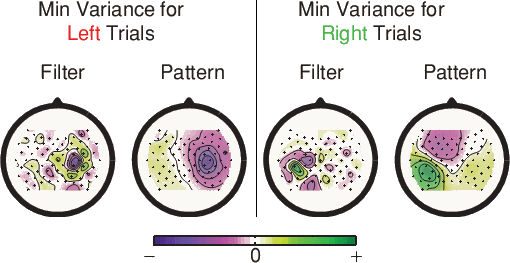
\includegraphics[scale=0.40]{topos.png} \\
\caption{Example of CSP analysis. The patterns illustrate how the presumed sources project to the scalp. They can be used to verify neurophysiological plausibility. The filters are used to project the original signals.}
\end{figure}

\section{Classification}
\subsection{Basic Classification Pipeline}
Now that we have learned about how to measure EEG-data, what  Event Related Synchronizations and Desynchronizations are and how to preprocess our data to make use of them, we want to put it all together and describe a simple classification pipeline. We will still focus on the task of classifying left- against right-hand movement.
So let's say, we have fetched some labeled epochs of EEG-data by instructing a participant to imagine his left or right hand moving and slicing out the corresponding EEG-data afterwards. For example we could take a 4-seconds window right after the instruction. We can now bandpass these epochs to an interesting frequency range, for example 8-13 Hz, and train CSP-filters on the estimated covariance matrices. In the final step, we can then train a classifier on the mean power of these virtual channels. For example Linear Discriminant Analysis has proven to give good results in this use case.

After this calibration and training phase, this obtained pipeline can then be used to classify between left- and right-hand movement in an online application. A window of the same length as our sample epochs can be slided over the EEG-signal. This window can then be bandpassed and filtered with the trained CSP-channels. We can then proceed to calculate the mean power of these channels and use our classifier to predict left or right. This output can then be used in an application to give feedback to the user and operate on given tasks.

\subsection{Results and Application}
With a similar method as the above described, the authors of [1] have achieved an average accuracy for left- and right-hand classification of over 90\%. 

This is already a pretty good rate for a wide spectrum of tasks ranging from fields like stroke rehabilitation to computer gaming. For example in [6] the authors describe several promising setups, where the imagery of movement was used to give haptic feedback to patients with disabilities caused by strokes. For a further overview of possible use cases of this type of brain computer interface, again a look into [2] is a good starting point.

\subsection{Possible Enhancements}
The just presented approach for classification ERD/ERS effects is a very basic one. Still, as already noted, this pipeline has some hyperparameters, that need to be tuned. We have to choose
\begin{itemize}
\item[1] The length and time point of the training epochs
\item[2] The range of bandpass filtering before training CSP-filters
\item[3] Selection of filters we want to use for classification
\item[4] Additional hyperparameters introduced by the model we opt for
\end{itemize}
With our approach we just guessed values, but there are interesting heuristic approaches for searching optimal parameters. For 1. to 3. these are also described in [1].

Secondly, it is possible to train filters and classifier on more than one part of the frequency range. We could for example choose to train in the $\mu$-range from 8-13 Hz like before and additionally train filters in the $\beta$-range from 20 to 30 Hz. Figure 3 indicates, that this might add to discriminability, as the $r^2$-score has a peak in that range, too.

Another clarification, that should be made, is that with this approach we are not bound to do two-class discrimination. We can use multiple classifying pipelines as the above on different classes and in that way create a setup, where we can classify between more than just left- and right-hand movement.

In general, if the reader is interested in further discussion of improvements, a look at the other contributions to this seminar, that can be found in [8], is recommended.

%----------------------------------------------------------------------------------------
%	REFERENCE LIST
%----------------------------------------------------------------------------------------

\begin{thebibliography}{99} % Bibliography - this is intentionally simple in this template
	\bibitem[1]{} Blankertz B, Tomioka R, Lemm S, Kawanabe M, Mueller KR, Optimizing Spatial Filters for Robust EEG Single-Trial Analysis. IEEE Signal Process Mag, 25(1):41-56, 2008.
	\bibitem[2]{} Wolpaw, Brain-Computer Interfaces: principles and practice. Oxford Univ. Press, 2011.
	\bibitem[3]{} mne$\-$tools.github.io/dev/auto$\_$examples/decoding/ \\ plot$\_$decoding$\_$csp$\_$eeg.html
	\bibitem[4]{} Schalk, G McFarland, DJ Hinterberger T, Birbaumer N, Wolpaw JR, BCI2000: A General-Purpose Brain-Computer Interface (BCI) System. IEEE TBME 51(6):1034-1043, 2004
	\bibitem[5]{} Introduction to Modern Brain-Computer Interface Design - Christian A. Kothe Swartz Center for Computational Neuroscience, University of California San Diego
	\bibitem[6]{} Cuntai Guan, Kai Keng Ang, Christopher Kuah, Effie Chew, Karen Chua: Brain-Computer Interface for Stroke Rehabilitation, 2014
	\bibitem[7]{} Benjamin Blankertz, Guido Dornhege, Matthias Krauledat, Gabriel Curio, and Klaus-Robert Mueller. The non-invasive Berlin Brain-Computer Interface: Fast acquisition of effective performance in untrained subjects.
NeuroImage, 37(2):539-550, 2007.
	\bibitem[8]{}http://www.bsdlab.uni-freiburg.de/teaching/sose18/seminar-proseminar-doing-by-thinking

\end{thebibliography}

%----------------------------------------------------------------------------------------

\end{document}
